\documentclass[14pt,hidelinks]{extarticle}

\usepackage[T2A]{fontenc}
\usepackage[utf8]{inputenc}
\usepackage[russian]{babel}
\usepackage{cmap}

\usepackage{xcolor}

\usepackage{helvet}
\usepackage{pscyr}


\usepackage{multicol}

% \usepackage{amssymb,amsfonts,amsmath,mathtext}
% \usepackage{cite,enumerate,float}

\graphicspath{{images/}}     % Подключаемые пакеты
%%% Макет страницы %%%
\geometry{a4paper,top=20mm,bottom=27mm,left=30mm,right=15mm}
\setstretch{1.15}

%%% Язык текста %%%
\selectlanguage{russian}

%%% Кодировки и шрифты %%%
\renewcommand{\rmdefault}{ftm} % Включаем Times New Roman

%%% Выравнивание и переносы %%%
\sloppy				% Избавляемся от переполнений
\clubpenalty=10000		% Запрещаем разрыв страницы после первой строки абзаца
\widowpenalty=10000		% Запрещаем разрыв страницы после последней строки абзаца
\interfootnotelinepenalty=10000 % Запрет разрывов сносок

%%% Нумерация страниц %%%
\fancypagestyle{empty}{%
\fancyhf{} % clear all header and footer fields
\renewcommand{\headrulewidth}{0pt}
\renewcommand{\footrulewidth}{0pt}
\setlength{\headheight}{5mm} 
}

\fancypagestyle{plain}{%
\fancyhf{} % clear all header and footer fields
\fancyfoot[R]{\thepage} 
\renewcommand{\headrulewidth}{0pt}
\renewcommand{\footrulewidth}{0pt}
\setlength{\headheight}{5mm}
}

\pagestyle{plain}

%%% Библиография %%%

\makeatletter
\bibliographystyle{ugost2003s} % Оформляем библиографию в соответствии с ГОСТ 7.1 2003

\let\oldthebibliography=\thebibliography
\let\endoldthebibliography=\endthebibliography
\renewenvironment{thebibliography}[1]{
  \begin{oldthebibliography}{#1}
    \setlength{\parskip}{0mm}
    \setlength{\itemsep}{0mm}
}
{
\end{oldthebibliography}
}

%%% Изображения %%%
\graphicspath{{images/}} % Пути к изображениям

%%% Содержание %%%
\renewcommand{\cfttoctitlefont}{\hfil \large\bfseries}

\setlength{\cftparskip}{0mm}
\setlength{\cftbeforesecskip}{0mm}
\setlength{\cftaftertoctitleskip}{14pt}

\renewcommand{\cftsecaftersnumb}{\:}
\renewcommand{\cftsecfont}{}   
\renewcommand{\cftsecpagefont}{\normalsize}
\renewcommand{\cftsecleader}{\cftdotfill{\cftdotsep}}
\setlength{\cftsecindent}{0mm}
\setlength{\cftsecnumwidth}{3mm}

\setlength{\cftsubsecindent}{4mm}
\setlength{\cftsubsecnumwidth}{8mm}

%%% Требования ЕСКД/СТП %%%

%%% Размеры заголовков
\newcommand{\sectionbreak}{\clearpage}

\titleformat{\section}{\large\bfseries}{\thesection}{\wordsep}{}
\titlespacing*{\section}{12mm}{14pt}{14pt}

\titleformat{name=\section,numberless}{\large\bfseries\filcenter}{}{0mm}{}
\titlespacing*{name=\section,numberless}{0mm}{14pt}{14pt}

\titleformat{name=\subsection}{\normalsize\bfseries}{\thesubsection}{\wordsep}{}
\titlespacing*{\subsection}{12mm}{14pt}{14pt}

\titleformat{name=\subsection,numberless}{\normalsize\bfseries}{}{0mm}{}
\titlespacing*{name=\subsection,numberless}{0mm}{14pt}{14pt}

%%% Нумерация параграфов

\counterwithout{paragraph}{subsubsection}
\counterwithin{paragraph}{subsection}
\renewcommand{\theparagraph}{\thesubsection.\arabic{paragraph}}
\setcounter{secnumdepth}{4}

\titleformat{name=\paragraph}[runin]{\normalsize\bfseries}{\theparagraph}{\wordsep}{}
\titlespacing*{\paragraph}{12mm}{14pt}{\wordsep}

%%% Размеры текста формул %%%

\DeclareMathSizes{12}{12}{6}{4}

%%% Расстояние между формулами

\AtBeginDocument{%
  \setlength\abovedisplayskip{14pt}%
  \setlength\belowdisplayskip{14pt}%
  \setlength\abovedisplayshortskip{14pt}%
  \setlength\belowdisplayshortskip{14pt}%
}

%%% Оформление текста

\setlength{\parskip}{0pt}
\setlength{\parindent}{12mm}

%%% Расстояние между плавающими элементами

\setlength{\floatsep}{14pt}     % between top floats
\setlength{\textfloatsep}{14pt} % between top/bottom floats and text
\setlength{\intextsep}{14pt}    % between text and float
\setlength{\dbltextfloatsep}{14pt}
\setlength{\dblfloatsep}{14pt}

 % костыль для того, чтобы убрать расстояние от картинки до текста
\setlength{\abovecaptionskip}{0pt}
\setlength{\belowcaptionskip}{0pt}
           
%%% Оформление списков
\AddEnumerateCounter{\asbuk}{\@asbuk}{\cyrm}

\setlist{nosep,listparindent=\parindent}
\setlist[1]{itemindent=18.5mm,leftmargin=0mm,itemsep=0mm,topsep=0mm,parsep=0mm}             
\setlist[itemize,1]{label=$-$}
\setlist[enumerate,1]{label=\arabic*)}

\setlist[2]{itemindent=20.5mm,leftmargin=0mm,itemsep=0mm,topsep=0mm,parsep=0mm}             

% Определяем новый стиль для списков,
% на которые есть ссылки в тексте
\newlist{reflist}{enumerate*}{1}
\setlist*[reflist,1]{%
  label=\asbuk*),
}

\setlist*[reflist,2]{%
  label=\arabic*),
}

%% Нумерация плавающих элементов

\counterwithin{figure}{section}
\counterwithin{table}{section}

\makeatletter
\AtBeginDocument{%
\renewcommand{\thetable}{\thesection.\arabic{table}}
\renewcommand{\thelstlisting}{\thesection.\arabic{lstlisting}}
\renewcommand{\thefigure}{\thesection.\arabic{figure}}
\let\c@lstlisting\c@figure}
\makeatother 

%% Подписи плавающих элементов

\captionsetup[figure]{
  labelsep=endash,
  justification=centering,
  singlelinecheck=false,
  position=bottom,
  skip=14pt}

\captionsetup[table]{
  labelsep=endash,
  justification=raggedright,
  singlelinecheck=false,
  position=top,
  skip=0mm}

\captionsetup[lstlisting]{
  labelsep=endash
}

\lstset{
basicstyle=\scriptsize\ttfamily,
numberstyle=\scriptsize\ttfamily,
keywordstyle=\bfseries,
commentstyle=\itshape,
numbers=left,
stepnumber=1,
frame=single,
resetmargins=true,
xleftmargin=7mm,
xrightmargin=2mm,
captionpos=b,
keepspaces=true,
breaklines=true,
aboveskip=22pt,
belowskip=10pt,
abovecaptionskip=16pt}

\renewcommand{\arraystretch}{1.5}

%%% Настройка размеров вертикальных отступов

\renewcommand{\smallskip}{\vspace{6pt}}
\renewcommand{\bigskip}{\vspace{14pt}}
	     % Пользовательские стили

\begin{document}

%%% Переопределение именований %%%
\renewcommand{\abstractname}{Аннотация}
\renewcommand{\alsoname}{см. также}
\renewcommand{\appendixname}{Приложение}
\renewcommand{\bibname}{Литература}
\renewcommand{\ccname}{исх.}
\renewcommand{\chaptername}{Глава}
\renewcommand{\contentsname}{СОДЕРЖАНИЕ}
\renewcommand{\enclname}{вкл.}
\renewcommand{\figurename}{Рисунок}
\renewcommand{\lstlistingname}{Рисунок}
\renewcommand{\headtoname}{вх.}
\renewcommand{\indexname}{Предметный указатель}
\renewcommand{\listfigurename}{Список рисунков}
\renewcommand{\listtablename}{Список таблиц}
\renewcommand{\pagename}{Стр.}
\renewcommand{\partname}{Часть}
\renewcommand{\seename}{см.}
\renewcommand{\tablename}{Таблица}

\renewcommand{\refname}{СПИСОК ИСПОЛЬЗОВАННЫХ ИСТОЧНИКОВ}
	     % Переопределение именований

%%%%%%%%%%%%%%%%%%%%%%%%%%%%%%%%%%%%%%%%%%%%%%%%%%%%%%%%%%%%%%%%

\begin{center}
	\textbf{Типовой расчет} \\ 
	выполнил ст. гр. ****** Петров Ю.А. \\
        Задача №11\\
	Вариант XX 
\end{center}

\section{Условие}

По выборке двумерной случайной величины:

\begin{itemize}
	\item вычислить оценку коэффициента корреляции;
        \item прлверить гипотезу об отсутствии \\
          корреляционной зависимости ($ \alpha = 0.05 $);
	\item вычислить параметры линии регрессии $ \alpha_0 $ и $ \alpha_1 $; 
	\item построить диаграмму рассеивания и линию регрессии;
\end{itemize}

Исходные данные для варианта XX приведены в таблице~\ref{tbl:second_sample}.

\begin{table}[h!]
  \renewcommand{\tabcolsep}{0.6em} 
	\centering
	\caption{Двумерная выборка\label{tbl:second_sample}}
	\begin{tabular}{llllllllll}
          -4.86	& -3.7	& -2.41	& -2.24	& -2.12	& -2.07	& -1.87	& -1.57	& -1.05	& -0.95	\\ 
-0.86	& -0.82	& -0.69	& -0.56	& -0.42	& -0.38	& -0.14	& -0.13	& -0.01	& 0.1	\\ 
0.13	& 0.41	& 0.46	& 0.53	& 0.7	& 0.84	& 0.99	& 1.06	& 1.19	& 1.21	\\ 
1.21	& 1.21	& 1.23	& 1.26	& 1.33	& 1.47	& 1.76	& 1.91	& 1.94	& 2.02	\\ 
2.09	& 2.12	& 2.2	& 2.22	& 2.24	& 2.37	& 2.38	& 2.45	& 2.51	& 2.6	\\ 
2.6	& 2.65	& 2.67	& 2.69	& 2.88	& 3.12	& 3.15	& 3.23	& 3.24	& 3.24	\\ 
3.26	& 3.44	& 4.09	& 4.09	& 4.47	& 4.79	& 4.95	& 5.01	& 5.03	& 5.18	\\ 
5.2	& 5.21	& 5.36	& 5.44	& 5.44	& 5.47	& 5.48	& 5.64	& 5.78	& 5.79	\\ 
5.81	& 5.94	& 5.98	& 6.11	& 6.49	& 6.54	& 6.63	& 6.75	& 7.05	& 7.13	\\ 
7.17	& 7.34	& 7.51	& 7.85	& 7.93	& 8.7	& 9.26	& 9.5	& 10.95	& 11.15	\\ 
	\\ 

	\end{tabular}
\end{table}

\newpage

\section{Решение}

\subsection{Вычисление точечных оценок параметров двумерной выборки}

Вычислим оценки математических ожиданий по каждой переменной.
\begin{align}
  m^*_X &= \overline{x} = \frac{1}{n} \sum_{i=1}^{n} x_i, &
  m^*_Y &= \overline{y} = \frac{1}{n} \sum_{i=1}^{n} y_i, \\ \nonumber
  m^*_X &= 0.1856, &
  m^*_Y &= 0.2122.
\end{align}

Вычислим оценки дисперсий по каждой переменной.
\begin{equation}
  \begin{aligned}
    D^*_X &= S^2_0(x) = \frac{1}{n-1} \sum_{i=1}^{n} (x_i - \overline{x})^2, \\
    D^*_Y &= S^2_0(y) = \frac{1}{n-1} \sum_{i=1}^{n} (y_i - \overline{y})^2,
  \end{aligned}
\end{equation} 
\begin{equation*}
  \begin{aligned}
    D^*_X &= 4.4893, &
    D^*_Y &= 3.3579.
  \end{aligned}
\end{equation*}

Вычислим оценку корреляционного момента:
\begin{equation}
  K^*_{XY} = \frac{1}{n-1} \sum_{i=1}^{n}{(x_i - \overline{x})(y_i - \overline{y})},
\end{equation} 
\begin{equation*}
  K^*_{XY} = 0.7663.
\end{equation*}

Найдем оценку коэффициента корреляции:
\begin{equation}
  R^*_{XY} = \frac{K^*_{XY}}{\sqrt{S^2_0(x) \cdot S^2_0(y)}},
\end{equation} 
\begin{equation*}
  R^*_{XY} = \dfrac{0.7663}
  {\sqrt{4.4893 \cdot 3.3579}} = 
  0.1974.
\end{equation*}

\subsection{Вычисление интервальной оценки коэффициента корреляции}

Вычислим интервальную оценку коэффициента корреляции с надёжностью $\gamma = 0.95$ по следующей формуле:
\begin{align}
  I_{\gamma} (R_{XY}) &= \left[ \frac{e^{2a}-1}{e^{2a}+1}; \frac{e^{2b}-1}{e^{2b}+1} \right]. 
\end{align}

Для этого в таблице функции Лапласа найдем значение, равное $\frac{\gamma}{2} = 0.475$ и определим значение аргумента, ему соответствующее:
\begin{equation*}
  z_{0.95} = arg \Phi (0.475) = 1.96. 
\end{equation*}

Для вычисления интервальной оценки коэффициента корреляции найдем вспомогательные значения $a, b$ по следующим формулам:
\begin{equation}
  \begin{aligned}
    a &= 0.5 \cdot ln \left( \frac{1+R^*_{XY}}{1-R^*_{XY}} \right) - \frac{z_{\gamma}}{\sqrt{n-3}}, \\
    b &= 0.5 \cdot ln \left( \frac{1+R^*_{XY}}{1-R^*_{XY}} \right) + \frac{z_{\gamma}}{\sqrt{n-3}}, \\
  \end{aligned}
\end{equation}
\begin{equation*}
  \begin{aligned}
    a &= -0.0859, &
    b &= 0.4859.
  \end{aligned}
\end{equation*}

Таким образом, доверительный интервал для коэффициента корреляции имеет вид:
\begin{align}
  I_{\gamma} (R_{XY}) &= \left[ \frac{e^{2a}-1}{e^{2a}+1}; \frac{e^{2b}-1}{e^{2b}+1} \right], \\ \nonumber
  I_{\gamma} (R_{XY}) &= \left[ -0.0857; 
    0.4509 \right]
\end{align}

\newpage 

\subsection{Проверка гипотезы об отсутствии корреляционной зависимости}
Выдвинем двухальтернативную гипотезу об отсутствии корреляционной зависимости 
между величинами $ X $ и $ Y $:

\begin{itemize}
\item $H_0$ --- $ R_{XY} = 0 $: между величинами $ X $ и $ Y $ корреляционная зависимость отсутствует;
\item $H_1$ --- $ R_{XY} \neq 0 $: между величинами $ X $ и $ Y $ существует корреляционная зависимость.
\end{itemize}

Так как объем выборки велик ($ n \ge 50 $), то вычислим значение критерия по формуле:
\begin{equation}
  Z = \dfrac{|R^*_{XY}| \cdot \sqrt{n}}{1-(R^*_{XY})^2},
\end{equation}
\begin{equation*}
  Z = 1.4236.
\end{equation*}

Определим значение $ Z_\alpha $ из таблицы функции Лапласа ($ \alpha = 0.05 $):
\begin{equation*}
  Z_{0.05} = 1.96.
\end{equation*}

\textbf{Вывод:} так как $ Z = 1.4236 {<}notation{>} Z_{0.05} $,
то гипотеза $H_0$ об отсутствии корреляционной зависимости между величинами $ X $ и $ Y $ принимается (отклоняется).

\newpage

\subsection{Построение линии регрессии}

Уравнение линии регрессии имеет следующий вид:
\begin{equation}
  \overline{y}(x) = a^*_0 + a^*_1 x,
\end{equation} 
где $a^*_1 = \dfrac{K^*_{XY}}{S^2_0(x)},\; a^*_0 = \overline{y} - a^*_1 \cdot \overline{x} $
--- коэффициенты линии регрессии.

\vspace{1em}
Найдем значения $ a^*_1, a^*_0 $:
\begin{equation*}
	\begin{aligned}
		a^*_1 &= 0.1707, &
		a^*_0 &= 0.1805
	\end{aligned}
\end{equation*}

Таким образом, линия регрессии примет вид:
\begin{equation}
  \overline{y}(x) = 0.1805
  + ( 0.1707 ) \cdot x
\end{equation}

График линии регрессии изображен на рисунке~\ref{fig:sample_regression}.
\begin{figure}[h!] 
  \centering
  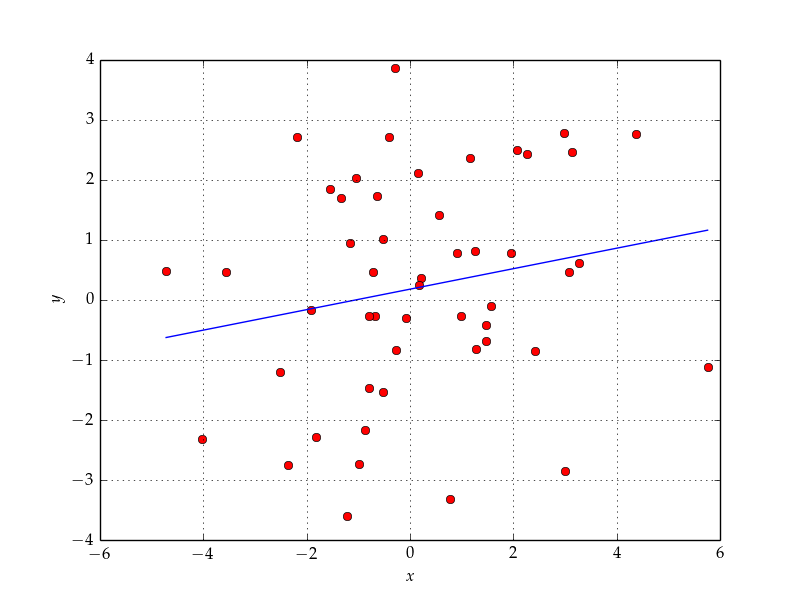
\includegraphics[width=1\linewidth]{pic/sample_regression}
  \caption{График линии регрессии для двумерной случайной величины\label{fig:sample_regression}}
\end{figure}


\end{document}